
\section{Introduction\label{introduction}}

The goal of automatic knowledge base construction (AKBC) is to build a structured knowledge base (KB) of facts using a noisy corpus of raw text evidence, and perhaps an initial seed KB to be augmented~\citep{NELL,yago,freebase}. AKBC supports downstream reasoning at a high level about extracted entities and their relations, and thus has broad-reaching applications to a variety of domains.

One challenge in AKBC is aligning knowledge from a structured KB with a text corpus in order to perform supervised learning through \emph{distant supervision}. \emph{Universal schema}~\citep{limin} along with its extensions~\citep{yao2013universal,vector_pra,neelakantan2015compositional,logicmfnaacl15}, avoids alignment by jointly embedding KB relations, entities, and surface text patterns. This propagates information between KB annotation and corresponding textual evidence.

The above applications of universal schema express each text relation as a distinct item to be embedded. This harms its ability to generalize to inputs not precisely seen at training time. Recently work \citep{toutanova2015representing,verga2015multilingual} has addressed this issue by embedding text patterns using a deep sentence encoder, which captures the compositional semantics of textual relations and allows for prediction on inputs never seen before.

While compositional universal schema has addressed the issue of unseen textual patterns, the problem of unseen entity pairs has not yet been resolved. Our solution is to remove explicit representations of entity pair vectors, and instead express each entity pair as a function of its mentions.


\subsection {Universal Schema}

Universal Schema embeds textual patters and knowledge bases into a shared space in order to reason over relations and entity pairs.
A low dimensional embedding is learned for each entity pair and each relation type using matrix factorization.
The model is then able to infer relations between entities as the dot product between the two entity pair and relation type vectors.

Unfortunately, this formulation limits the generalization of the model.

Recently Universal Schema has been extended to deal with compositional representations of textual relations \citep{toutanova2015representing,verga2015multilingual}
This gives us the ability to generalize to unseen textual patterns.

\begin{figure}[h]
\caption{Top : Universal Schema expresses each textual pattern as an atomic unit \protect\citet{riedel2010modeling}.
Bottom : Compositional Universal Schema uses an lstm to encode each textual relation \protect\cite{verga2015multilingual}. }
\centering
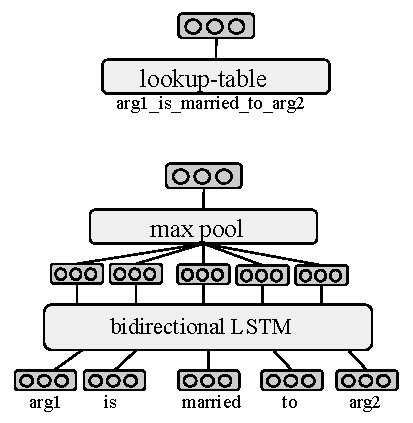
\includegraphics[scale=.68]{relation-models}
\end{figure}


\subsection {Entities vs Entity Pairs}

A knowledge base is naturally described as a graph, in which entities are nodes and relations are labeled edges~\citep{yago,freebase}.
In the case of \emph{knowledge graph completion}, the task is akin to link prediction, assuming an initial set of (\emph{s, r, o}) triples.
See~\citet{nickel2015review} for a review.
No accompanying text data is necessary, since links can be predicted using properties of the graph, such as transitivity.
In order to generalize well, prediction is often posed as low-rank matrix or tensor factorization.
A variety of model variants have been suggested, where the probability of a given edge existing depends on a multi-linear form~\citep{rescal,DBLP:journals/corr/Garcia-DuranBUG15,bishan,transe,wang2014knowledge,lin2015learning}, or non-linear interactions between $s$, $r$, and $o$~\citep{socherkb}.

These models all operate at the level of entities rather than entity pairs.
Entity-based models have recall advantages over entity pairs.
For any two entities, the model is able to make predictions even if there is no information regarding the explicit entity pair.
However, this essentially reduces to type clustering as every action star would have a high probability for every action movie.

Entity pairs on the other hand have higher precision.
Both~\citet{toutanova2015representing} and~\citet{limin} observed that the entity pair model outperforms entity models in cases where the entity pair was seen at training time.
This is particularly important when jointly embedding text and knowledge bases.
By leveraging large amounts of unlabeled text, Universal Schema is able to find additional textual evidence for entity pairs.
We are interested in high precision information extraction from direct textual provenance.


\subsection {Entities as Relations}

Rather than modeling each entity pair as an explicit vector, we instead treat each entity pair as an aggregate function over each of its relation types.
This allows us to trivially extend to unseen entity pairs, have a direct link to provenance, and allocate a variable number of parameters per entity pair.